\chapter{函数}
\label{funcchap}
\index{function call 函数调用}

在程序设计中,函数是带有函数名的一系列执行计算的语句,当定义一个函数,我们指
定一个函数名和一系列的语句。然后,就可以通过函数名调用函数。我们其实已经看到
一个函数调用的例子。

\beforeverb
\begin{verbatim}
>>>type(32)
<type 'int'>
\end{verbatim}
\afterverb

函数名是类型,小括号里的表达式称作函数的形式参数(argument).结果是形参的类型。

\index{parenthess!argument in}

通常我们这么说:函数接受一个参数,返回一个结果(叫做返回值)。

\index{argument 形式参数}
\index{return value 返回值}

\section{类型转换函数}
\index{conversion!type 转换!类型}
\index{type conversion 类型转换}

Python提供一些内置函数用来把一种类型的值转换成另一类型。{\\t int}函数接受一
个值,如果可以,就把它转换成整数,否则就会“抱怨”。

\index{int function int 函数}
\index{function!int 函数!int}

\beforeverb
\begin{verbatim}
>>> int('32')
32
>>> int('Hello')
Traceback (most recent call last):
  File "<stdin>", line 1, in <module>
ValueError: invalid literal for int() with base 10: 'Hello'
\end{verbatim}
\afterverb

{\tt int}函数可以把浮点数转换为整数,但是不能向上取整,只能截掉小数部分:

\beforeverb
\begin{verbatim}
>>> int(3.99999)
3
>>> int(-2.3)
-2
\end{verbatim}
\afterverb

{\tt float}函数把整数和字符串转换成浮点数:

\index{float function float函数}
\index{function!float 函数!float}

\beforeverb
\begin{verbatim}
>>>float(32)
32.0
>>>float('3.14159')
3.14159
\end{verbatim}
\afterverb \footnote{在译者的机器上float('3.14159')的输出为:3.1415899999999999(解释器Python2.5和2.6);3.14159(解释器Python3.1)。}

最后,{\tt str}把参数转换为字符串:

\index{str function str函数}
\index{function!str 函数!str}

\beforeverb
\begin{verbatim}
>>>str(32)
'32'
>>>str(3.14159)
'3.14159'
\end{verbatim}
\afterverb




\section{数学函数}
\index{math function 数学函数}
\index{function, math 函数,数学}

Python带有一个数学模块,提供了大多数我们熟悉的数学函数。模块是一个包含一系列有联系函数的文件。

\index{module 模块}
\index{module object 模块对象}

在我们使用模块之前,必须导入它。

\beforeverb
\begin{verbatim}
>>>import math
\end{verbatim}
\afterverb

这个语句创建了一个叫做math的模块对象。如果你尝试打印模块
对象,你会得到如下的信息:

\beforeverb
\begin{verbatim}
>>>print math
<module 'math' from '/usr/lib/python2.5/lib-dynload/math.so'>
\end{verbatim}
\afterverb

模块对象包含了定义在该模块内的函数和变量。要访问这些
函数,你必须指定模块名和函数名,中间用“.“分隔。这种格式叫做点记法。

\index{dot notation 点记法}

\beforeverb
\begin{verbatim}
>>>ratio = signal_poewe / noise_poewr
>>>decibels = 10 * math.log10(ratio)

>>>radians = 0.7
>>>height = math.sin(radians)
\end{verbatim}
\afterverb

第一个例子计算以10为底,信噪比的对数。math模块也提供了
{\tt log}来计算以{\tt e}为底的对数。

\index{log function log函数}
\index{function!log 函数!log}
\index{sine function sin函数}
\index{radian 弧度}
\index{trigonometric function 三角函数}
\index{function, trigonometric 函数, 三角}

第二个例子计算{\tt radians}的正弦值。变量名提示{\tt sin}和
其他的三角函数({\tt cos},{\tt tan} 等等)接受弧度作为参数。
度除以360,再乘以$2\pi$,就得到弧度。

\beforeverb
\begin{verbatim}
>>>degrees = 45
>>>radians = degrees / 360.0 * 2 * math.pi
>>>math.sin(radians)
0.707106781187
\end{verbatim}
\afterverb \footnote{在译者的机器上输出为:0.70710678118654746}

表达式{\tt math.pi}从math模块获得变量{\tt pi}。变量{\tt pi}的值近似等于$\pi$,精度大约达到15个位。

\index{pi}

如果了解三角学,你可以拿上面的结果和二分之根号二比较,看看是否相等:

\index{sqrt function sqrt函数}
\index{function!sqrt 函数!sqrt}


\beforeverb
\begin{verbatim}
>>>math.sqrt(2) / 2.0
0.707106781187
\end{verbatim}
\afterverb \footnote{在译者的机器上,两者只能是近似相等,计算机对浮点数的处理都会涉及到精度问题}


\section{创建}
\index{创建}

迄今为止,我们已经见到了程序的部分元素---变量,表达式,语句---并
没有把他们结合起来,而只是孤立的涉及到。\\

程序设计语言最强大的一个特色就是能够把小块的程序块结合起来,创建一个程序块。比如,函数的参数可以是任何表达式,包括数学运算符:

\beforeverb
\begin{verbatim}
x = math.sin{degrees / 360 * 2 * math.pi)
\end{verbatim}
\afterverb

甚至包括函数调用:

\beforeverb
\begin{verbatim}
x = math.exp(math.log(x+1))
\end{verbatim}
\afterverb

	
可以这么说,可以接受值的地方,几乎都可以放置一个表达式。有一个例外:赋值语句的左面必须是一个变量名。\footnote{在c/c++中,叫做左值}。其他的任何表达式放在左面都会引起语法错误\footnote{我们即将看到这样的异常}。

\beforeverb
\begin{verbatim}
>>>minutes = hours * 60   # 正确
>>>hours * 60 = minutes   # 错误!
SyntaxError: can't assign to operator
\end{verbatim}
\afterverb

\index{SyntaxErrot 语法错误}
\index{exception!SyntaxError}


\section{编写新的函数}

直到现在,我们只是使用Python自带的函数,当然,我们也可以
编写自己的新函数。函数定义指明了当函数被调用时,新函数的名
字和一系列的语句集合。

\index{function 函数}
\index{function definition 函数定义}
\index{definition!function 定义!函数}

这儿有个例子:

\beforeverb
\begin{verbatim}
def print_lyrics():
	print "I'm a lumberjack, and I'm okay."
	print "I sleep all night and I work all day."
\end{verbatim}
\afterverb

{\tt def}是一个关键字,表明这是一个函数定义。函数名是\verb"print_lyrics"。函数名的命名规则和变量名一样:字母,数字和一些标点符号是合法的,但是首字符不可以是数字。我们也不可以用关键字作为函数的名字,并且也要尽量避免函数和变量使用相同的名字。\\

\index{def keyword def关键字}
\index{keyword!def 关键字!def}
\index{argument 参数}

函数名后面的空的小括号表明,函数不带有任何参数。
\index{parentheses!empty 小括号!空}
\index{header 头}
\index{body 体}
\index{indentation 缩进}
\index{colon 分号}

函数定义的第一行叫做函数头;其余的部分叫做函数体。函数头必须要
以一个分号结尾,函数体必须要有缩进。通常,缩进四个空格(参看 
Section~\ref{编辑器})。函数体可以包含任意数量的语句。\\
	
print语句的字符串是用双引号引起来的。单引号好双引号效果是一样的;大多数的人使用单引号,除了单引号也出现在字符串中。
\index{ellipses 省略号}

如果在交互模式下输入函数,解释器输出省略号({\em ...})让我们
获悉函数定义还没有结束:

\beforeverb
\begin{verbatim}
>>> def print_lyrics():
...     print "I'm a lumberjack, and I'm okay."
...     print "I sleep all night and I work all day."
...
\end{verbatim}
\afterverb

要结束一个函数定义,必须留有一个空行(在脚本模式下无须若此)。\\

定义一个函数,也就创建了同名的变量。

\beforeverb
\begin{verbatim}
>>> print print_lyrics
<function print_lyrics at 0xb7e99e9c>
>>> print type(print_lyrics)
<type 'function'>
\end{verbatim}
\afterverb

\verb"print_lyrics"的值是一个函数对象,类型是\verb"'function'"。

\index{function object 函数对象}
\index{object!function 对象!函数}

调用自建的函数和内置函数的语法是相同的:

\beforeverb
\begin{verbatim}
>>> print_lyrics()
I'm a lumberjack, and I'm okay.
I sleep all night and I work all day.
\end{verbatim}
\afterverb

一旦定义了一个函数,就可以在其他函数中使用它。比如,要重复前面的打印的话,我们可以写一个函数,叫\verb"repeat_lyrics":

\beforeverb
\begin{verbatim}
def repeat_lyrics():
    print_lyrics()
    print_lyrics()
\end{verbatim}
\afterverb

 再调用之:

 \beforeverb
\begin{verbatim}
>>> repeat_lyrics()
I'm a lumberjack, and I'm okay.
I sleep all night and I work all day.
I'm a lumberjack, and I'm okay.
I sleep all night and I work all day.
\end{verbatim}
\afterverb

但是,真实的歌儿可不是这么唱的~~。


\section{定义和使用}
\index{function definition 函数定义}

组合一个前面的代码片段,真个的程序看上去是这样的:

\beforeverb
\begin{verbatim}
def print_lyrics():
    print "I'm a lumberjack, and I'm okay."
    print "I sleep all night and I work all day."

def repeat_lyrics():
    print_lyrics()
    print_lyrics()

repeat_lyrics()
\end{verbatim}
\afterverb

这个程序包含了两个函数定义:\verb"print_lyrics"和\verb"repeat_lyrics"。函数定义的执行就像其他语句一样,只是创建的是一个函数对象。函数体里的语句知道函数被调用的时候才执行,函数调用也不产生任何输出。

\index{use before def定义前使用}

 正如期待的,在使用前,我们必须创建一个函数。还句话说,函数定义
 在第一次调用前必须被执行。

 \begin{ex}
 把上面程序最后以行移到顶部,这样,函数调用在定义前出现。运行
 程序,看看有什么错误信息输出。
 \end{ex}

 \begin{ex}
 再把函数调用移到底部,并且把\verb"print_lyrics"函数定义移到\verb"repeat_lyrics"后面。再运行程序,看看有什么输出?
 \end{ex}


\section{执行流}
\index{flow of execution 执行流j}

为了保证函数在第一次使用前定义,我们必须知道语句的执行顺序,叫做
执行流。\\

执行通常是从程序的第一个语句开始的。语句一次执行一句,自顶向下。\\

函数调用就像一次执行流的迂回。不是执行下一个语句,执行流跳转到
函数体里,执行那里的所有语句,然后再会到上次跳转的地方。\\

这听起来很简单,但是还记得我们说过函数也是可以调用其他函数的?当
执行流在一个函数的中间时,程序可能不得不执行另外一个函数的语句。
当执行那个新的函数时,程序可能不得不执行其他另外一个函数!\\

幸运的是,Python很擅长追踪执行流在哪里,所以,每次函数执行完成
时,程序回到调用它的函数的调用点。当到达程序末尾时,执行流终止。\\

这个“混乱不堪”的叙述的寓意是什么呢?当你读程序的时候,不必要从上至下。有时候,按着执行流读,甚至更有意义。

\section{形参和实参}
\label{parameters}
\index{parameter 形参}
\index{function parameter 函数形参}
\index{argument 实参}
\index{function argument 函数实参}

我们已经见到一些内置函数需要接受实参。比如,当调用{\tt math.sin}
,我们传递一个数字作为实参。一些函数接受不止一个参数:{\tt math.pow}接受两个,底和幂:

\index{parentheses!parameters in}

\beforeverb
\begin{verbatim}
def print_twice(bruce):
    print bruce
    print bruce
\end{verbatim}
\afterverb

这个函数,把实参赋值给形参{\tt bruce}。当函数被调用时,打印形参
的值两次(无论是什么)。\\

函数接受任意可被打印的值。

\beforeverb
\begin{verbatim}
>>> print_twice('Spam')
Spam
Spam
>>> print_twice(17)
17
17
>>> print_twice(math.pi)
3.14159265359
3.14159265359
\end{verbatim}
\afterverb

适用于内置函数的创建规则同样也适用于用户自定义函数,由此,我们可以使用任何表达式作为\verb"print_twice"的实参:

\index{composition 创建}

\beforeverb
\begin{verbatim}
>>> print_twice('Spam '*4)
Spam Spam Spam Spam
Spam Spam Spam Spam
>>> print_twice(math.cos(math.pi))
-1.0
-1.0
\end{verbatim}
\afterverb


实参在函数调用开始前被计算,所以,在例子中,表达式\verb"'Spam '*4"和{\tt math.cos(math.pi)}只被计算一次。\\

\index{argument 实参}

也可以用一个变量作为实参:

\beforeverb
\begin{verbatim}
>>> michael = 'Eric, the half a bee.'
>>> print_twice(michael)
Eric, the half a bee.
Eric, the half a bee.
\end{verbatim}
\afterverb


我们作为实参传递给函数的变量名({\tt michael})和形参({\tt bruce})没有任何关系。每个值的名称是无所谓的(在调用函数中),
在\verb"print_twice",我们把每个人叫做{\tt bruce}。

\section{变量和参数是局部的}
\index{local variable 局域变量}
\index{variable!local 变量!局域}

当在函数中创建一个变量,它是局域,意味着它只存在于函数中。比如:

\index{Parentheses!parameters in}

\beforeverb
\begin{verbatim}
def cat_twice(part1, part2):
    cat = part1 + part2
    print_twice(cat)
\end{verbatim}
\afterverb

函数接受两个参数,连接它们,打印结果两次。请看下面的实例:

\index{concatenation 连接}

\beforeverb
\begin{verbatim}
>>> line1 = 'Bing tiddle '
>>> line2 = 'tiddle bang.'
>>> cat_twice(line1, line2)
Bing tiddle tiddle bang.
Bing tiddle tiddle bang.
\end{verbatim}
\afterverb

当\verb"cat_twice"结束的时候,变量{\tt cat}就毁灭了。如果我们尝试打印它,我们会得到一个异常:

\index{NameError}
\index{exception!NameError}

\beforeverb
\begin{verbatim}
>>> print cat
NameError: name 'cat' is not defined
\end{verbatim}
\afterverb

形参也是局域的。比如, 在\verb"print_twice"外,没有{\tt bruce}这个东东。

\index{parameter 形参}

\section{Stack diagrams 堆栈示意图}
\label{stackdiagram}
\index{stack diagrams 堆栈示意图}
\index{function frame 函数框}
\index{frame 框架}

为了跟踪哪个变量可以在哪里使用,有时,画堆栈示意图是非常有效的。
像状态图一样,堆栈图显示了每个变量的值,同时也显示了变量所属的函数。

\index{stack diagram 堆栈示意图}
\index{diagram!stack}

每个框图代表一个函数。一个框图就是一个盒子,旁边是函数名,里面是
函数形参和变量。我们可以把前面的例子表示成框图:

\beforefig
\centerline{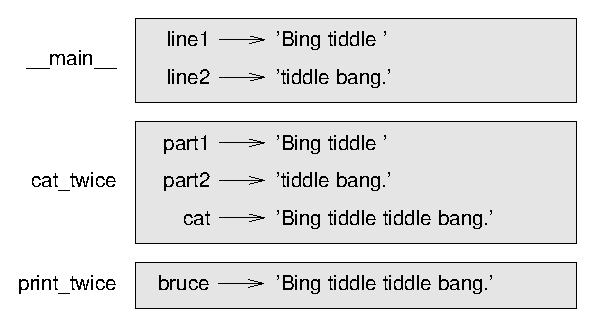
\includegraphics{figs/stack.eps}}
\afterfig

框图被安排在堆栈中,表明哪个函数调用哪个函数。在这个例子中,\verb"print_twice"被\verb"cat_twice"调用,\verb"cat_twice"被\verb"__main__"调用。 \\

每一个形参指向和他相关联的实参的值。所以,{\tt part1}和{\tt line1}拥有相同的值,{\tt part2}和{\tt line2}拥有相同的值,{\tt bruce}和{\tt cat}拥有相同的值。\\

如果在函数调用过程中出现错误,Python打印函数的名称,调用它的函数的函数名,和上一个调用它的函数,一知道\verb"__main__"函数。
比如,如果尝试在\verb"print_twice"函数里访问{\tt cat},将会得到
一个{\tt NameError}:

\beforeverb
\begin{verbatim}
Traceback (innermost last):
  File "test.py", line 13, in __main__
    cat_twice(line1, line2)
  File "test.py", line 5, in cat_twice
    print_twice(cat)
  File "test.py", line 9, in print_twice
    print cat
NameError: name 'cat' is not defined
\end{verbatim}
\afterverb

这样列举函数叫做{\bf traceback}(追踪)。它告诉我们错误发生在哪个文件,哪行,当时哪个函数在执行。也显示了引起错误的行号。

\index{traceback 追踪}

在{\tt traceback}中的函数顺序和在堆栈图中的框图是一样的。正在运行的函数在最底部。

\section{“结果”函数和void 函数}

\index{fruitful function 卓有成效的函数}
\index{void function void 函数}
\index{function, fruitful}
\index{function, void}

一些我们使用的函数,比如math函数,产生结果;找不到一个更好的名字
,我姑且称他为“结果函数”({\bf fruitful functions})。其他函数,像\verb"print_twice",实施一个动作,但是没有返回一个值。他们叫做“虚无函数“({\bf void function})\footnote{译注:这些只是作者自己的命名}。  \\

当调用一个“结果函数“时,你大多数情况下希望对返回结果做些什么;比如,你可能把它赋给一个变量或者把它作为一个表达式的一部分:

\beforeverb
\begin{verbatim}
x = math.cos(radians)
golden = (math.sqrt(5) + 1) / 2
\end{verbatim}
\afterverb

当你在交互模式调用一个函数,Python显示如下结果:

\beforeverb
\begin{verbatim}
>>> math.sqrt(5)
2.2360679774997898
\end{verbatim}
\afterverb

但在脚本中,如果,调用仅仅调用一个“结果函数”,返回值就永远的丢失了!

\beforeverb
\begin{verbatim}
math.sqrt(5)
\end{verbatim}
\afterverb

脚本计算5的平方根,但是因为它不存储或者显示结果,所以没有多大的价值\footnote{译注:可以作为一条语句执行,这就是它的价值}。

\index{interactive mode 交互模式}
\index{script mode 脚本模式}

虚无函数({\tt Void 函数})在屏幕上显示某些东西,或者产生其他的效果,但是他们没有返回值。如果尝试着把结果赋给一个变量,我们将会得到一个特殊的值{\tt None}。

\index{None special value None特殊值}
\index{special value!None}

\beforeverb
\begin{verbatim}
>>> result = print_twice('Bing')
Bing
Bing
>>> print result
None
\end{verbatim}
\afterverb

{\tt None}的值和字符串\verb"'None'"是截然不同的概念。它有一个
特殊的类型:

\beforeverb
\begin{verbatim}
>>> print type(None)
<type 'NoneType'>
\end{verbatim}
\afterverb

截至目前,我们写的函数都是“虚无函数",再过几章,我们就开始编写“
结构函数”。

\section{为什么要函数}
\index{function, reason for}

可能大家还不是很清楚,为什么我们要花大力气去把程序分割成函数。有以下几个原因:

\begin{itemize}

\item 创建一个新函数,让我们有机会去给一组语句命名,这使得程序易读和易调试。

\item 通过消除重复的代码,函数可以使程序变得精巧。以后,如果想做
个改动,只需要改变一个地方。

\item 把一个规模庞大的程序分解成函数使得我们一次调试一个地方,然
后把他们组合起来,成为一个可工作的整体。

\item 设计良好的函数在很多程序中都会有用武之地。一旦写了一个,调
试无误,就可以重用\footnote{译注:reuse,有的书上建议翻译成复用
}。

\end{itemize}

\section{调试}
\label{editor}
\index{debugging 调试}


如果使用编辑器编辑脚本,可能会遇到空格符和制表符的问题。避免这些
问题最好的方式就是只使用空格(不用制表)。大多数的编辑器(对Python支持)默认使用这个方式,但是有一些不是。

\index{whitespace 空白}

制表符和空格符一般都是不可见的,这使得他们很难去调试,所以,最好
使用能够自动为你产生缩进的编辑器\footnote{译注:译者最喜欢的编辑
器Vim和Geany对Python的支持都是非常好的}。\\

另外,别忘了在运行程序之前,保存它。有些开发环境自动保存,但是有
些不\footnote{译注:一般,编辑器都是可以设置成自动保存的}。如果
没有保存, 你在编辑器里看到的程序和你运行的可能不是一样的。\\

一定要确保你看到的代码就是你要运行的代码。如果不确定的话,在程序
开始加入一些语句,比如\verb"print 'hello'",重新运行之。如果你
没有看到\verb"hello", 你运行的就不是你想要的程序。


\section{术语表}

\begin{description}

\item[function 函数:] 带有名字的,执行有意义的操作的语句集合。
函数可以接受也可以不接受参数和产生结果。
\index{function 函数}


\item[functon definition 函数定义:] 一个创建新函数的语句,指明
了函数名,参数,和执行的语句。
\index{function definition 函数定义}

\item[function object 函数对象:] 由函数定义常见的值。函数名就是一个指向函数对象的变量。
\index{function object 函数对象}

\item[header 函数头:] 函数定义的第一行。
\index{header 函数头}

\item[body 函数体:] 函数定义里面的一系列语句。
\index{body 函数体}

\item[parameter 形参:] 函数里指向传递过来的实参值的一个名字。
\index{parameter 形参}

\item[function call 函数调用:]一条执行函数的语句。由函数名和一
个参数列表组成。
\index{function call 函数调用}

\item[argument 实参:] 函数被调用时,提供给函数的值。这个值被赋
给函数里相应的形参。
\index{argument 实参}

\item[local variable 局域变领:]定义在函数里的变量。只能在函数体里使用。
\index{local variable 局域变量}

\item[return value 返回值:]函数的结果。如果函数调用被用作表达式
,返回值是表达式的值。
\index{return value 返回值}

\item[fruitful function 结果函数:]有返回值的函数。
\index{fruitful fucntion 结果函数}

\item[void function 虚无函数:]没有返回值的函数。
\index{void function 虚无函数}

\item[module 模块:] 包含一系列函数和其他定义的文件。
\index{module 模块}

\item[import statement import语句:] 读取模块文件,创建模块对象
的语句。
\index{import statement import语句}
\index{statement!import}


\item[module object 模块对象:]由{\tt import}语句创建的值,提供
了访问定义在模块里值的能力。
\index{module 模块}

\item[dot notation 点记法:]调用另外一个模跨函数的语法,具体的是
模块名后加一个点,让后是函数名。
\index{dot notation 点记法}

\item[composition 创建:]用一个表达式作为更大表达式的一部分,或
者一个语句作为更大语句的一部分。
\index{compositon 创建}

\item[flow of execution 执行流:]程序运行期间,语句的执行顺序。

\index{flow of execution 执行流}

\item[stack diagram 堆栈图:]函数,及其变量和制的图式化堆栈表示。
\index{stack diagram 堆栈图}

\item[frame 框图:] 堆栈图中的盒子,用来表示一个函数调用。包含
了函数的局部变量和形式参数。
\index{function frame 函数框图}
\index{frame 框图}

\item[traceback:] 异常发生时,打印的正在执行的函数表。
\index{traceback}

\end{description}


\section{练习}

\begin{ex}
\index{function!len}

Python提供了内置函数{\tt len},返回字符串的长度,\verb"len('allen')"的值是5。\\

编写一个名为\verb"right_justify"的函数,接受一个名为{\tt s}的参数,打印该字符串,使得打印的字符串的最后一个字符在第70列。

\beforeverb
\begin{verbatim}
>>> right_justify('allen')
                                                                 allen
\end{verbatim}
\afterverb

\end{ex}


\begin{ex}
\index{function object 函数对象}
\index{object!function}

函数对象是一个值,所以你可以把它赋给一个变量,或者把它作为参数
传递。比如,\verb"do_twice"函数接受一个函数对象作为参数,然后调用两次:

\beforeverb
\begin{verbatim}
def do_twice(f):
    f()
    f()
\end{verbatim}
\afterverb

这里是另外一个例子,使用\verb"do_twice"调用函数\verb"print_spam"两次。

\beforeverb
\begin{verbatim}
def print_spam():
    print 'spam'

do_twice(print_spam)
\end{verbatim}
\afterverb

\begin{enumerate}

\item 把上面的例子输入脚本,测试一下。

\item 修改\verb"do_twice"函数,让它接受两个参数---一个函数对象和
一个普通的值,调用函数两次,把普通值作为实参。

\item 编写一个更一般版本的\verb"print_spam",调用\verb"print_twice"两次,传递\verb"'spam'"作为实参。

\item 定义一个新的函数\verb"do_four",就手一个函数低相和一个普通值,调用函数四次,传递普通值给函数,作为参数。函数体里只能有两个
语句,不能有四个。

\end{enumerate}

你可以参考我提供的答案\url{thinkpython.com/code/do_four.py}。

\end{ex}


\begin{ex}

这个练习\footnote{基于Oualline的一个练习,{\em Practical C Programming, Third Edition},O'Reilly(1997)}可以只用我们迄今为止学过的
语句和其他语言特点实现。

\index{grid 网格}

\begin{enumerate}

\item 编写一个函数,打印如下的网格:

\beforeverb
\begin{verbatim}
+ - - - - + - - - - +
|         |         |
|         |         |
|         |         |
|         |         |
+ - - - - + - - - - +
|         |         |
|         |         |
|         |         |
|         |         |
+ - - - - + - - - - +
\end{verbatim}
\afterverb

提示:要在一行打印多个值,可以打印一个逗号分隔的语句序列:

\beforeverb
\begin{verbatim}
print '+', '-'
\end{verbatim}
\afterverb
%

如果序列以逗号结尾,Python会认为此句没有结束,所以打印的值在同
一行。
\beforeverb
\begin{verbatim}
print '+', 
print '-'
\end{verbatim}
\afterverb
%

语句的输出是\verb"'+-'"。


{\tt print}语句自动结束本行,进入下一行。

\item 是哦嗯先前的函数打印类似的网格,要求4行4列。

\end{enumerate}

可以参考我的答案:\url{thinkpython.com/code/grid.py}。

\end{ex}















































1


